\documentclass[compress,color=usenames]{beamer}

\newcommand{\mytitlenbr}{1}
\newcommand{\mytitle}{Image Archive}

%\documentclass[compress,color=usenames,handout]{beamer}

%\usepackage{pgfpages}
%\pgfpagelayout{4 on 2}[a4paper,border shrink=5mm]

\usepackage{graphicx}
\usepackage{amsfonts,amssymb}
\usepackage{latexsym}
\usepackage{mdwtab}
\usepackage{xspace}
\usepackage{tikz}
\usetikzlibrary{shapes,snakes}
\usetikzlibrary{petri}

\DefineNamedColor{named}{Periwinkle}{cmyk}{0.57,0.55,0,0}
\DefineNamedColor{named}{Plum}{cmyk}{0.50,1,0,0}
\DefineNamedColor{named}{Red}{cmyk}{0,1,1,0}

\newcommand{\mH}[1]{\textcolor{Plum}{#1}}
\newcommand{\mT}[1]{\textcolor{Periwinkle}{#1}}

\newcommand{\tup}[1]{\langle #1 \rangle}

\newcommand{\dd}{{:}}
\newcommand{\I}{\mathcal{I}}
\newcommand{\csetsc}[2]{\{#1 \mid #2\}}
\newcommand{\cset}[1]{\{#1\}}

\newcommand{\CON}{\textsf{CON}\xspace}
\newcommand{\ROL}{\textsf{ROL}\xspace}
\newcommand{\IND}{\textsf{IND}\xspace}
\newcommand{\PROP}{\textsf{PROP}\xspace}
\newcommand{\lang}{\mathcal{L}\xspace}

\newcommand{\mytt}[1]{\textsf{\scriptsize{#1}}}
\newcommand{\mytts}[1]{\textsf{\scriptsize{#1}}}

%\usefonttheme{serif}

\mode<presentation>
 {
 \usetheme{lined}
 }

\setbeamertemplate{navigation symbols}{}

\newcommand{\F}{\mathop{\mathsf{F}\vphantom{a}}\nolimits}
\newcommand{\G}{\mathop{\mathsf{G}\vphantom{a}}\nolimits}
\newcommand{\X}{\mathop{\mathsf{X}\vphantom{a}}\nolimits}

\newcommand{\Blue}[1]{\textcolor{blue}{#1}}
\newcommand{\Red}[1]{\textcolor{red}{#1}}
\newcommand{\Green}[1]{\textcolor{PineGreen}{#1}}

\title[GLN y Aplicaciones]{\Huge Generaci\'on de Lenguaje Natural y Aplicaciones}
%\mH{Lecture \#\mytitlenbr:} \mytitle}

\author[Areces \& Benotti]{
 Carlos Areces y Luciana Benotti\\[1ex]
\normalsize \url{{carlos.areces, luciana.benotti}@gmail.com}}

\institute[INRIA / UNC]{
INRIA Nancy Grand Est, Nancy, France\\
Universidad Nacional de C\'ordoba, C\'ordoba, Argentina}

\date{ELiC 2010 - Buenos Aires - Argentina}

\begin{document}

\beamerdefaultoverlayspecification{}

\begin{frame}[plain]
 \titlepage
\end{frame}

\begin{frame}
\frametitle{Lo que Vemos Hoy}

\begin{itemize}
\item \mH{TAGs y Surface Realization}
\item Generaci\'ion de Expresiones Referenciales
\end{itemize}
\end{frame}

\begin{frame}
\frametitle{Lo que Vemos Hoy}

\begin{itemize}
\item \mH{TAGs y Surface Realization}
\begin{tabular}{|l}
Inteface sint\'axis / sem\'antica\\
Algoritmo de Realizaci\'on
\end{tabular}
\item Generaci\'on de Expresiones Referenciales
\end{itemize}
\end{frame}

\begin{frame}
\frametitle{Substituci\'on}

\begin{center}
\begin{tabular}{|c|c|} \hline
From & We obtain \\ \hline

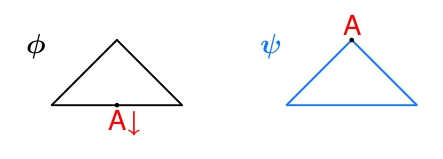
\includegraphics[scale=.4]{pics/pic2-17.jpg} & 

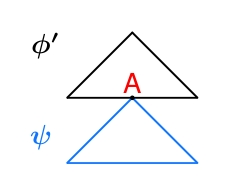
\includegraphics[scale=.4]{pics/pic2-18.jpg} \\ \hline

\multicolumn{2}{|c|}{by substituci\'on}  \\ \hline
\end{tabular}
\end{center}\pause


\mH{Ejemplo:}\begin{tabular}{l}
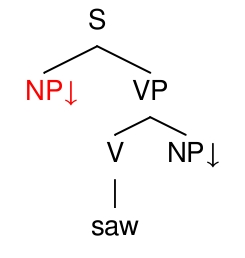
\includegraphics[scale=.4]{pics/pic2-19.jpg} \ \ \ \ \ \
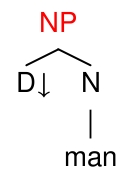
\includegraphics[scale=.4]{pics/pic2-20.jpg} \ \ \ \ \ \ 
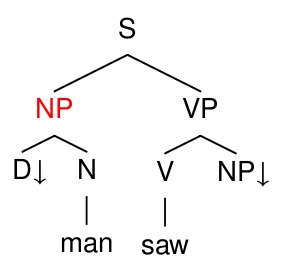
\includegraphics[scale=.4]{pics/pic2-21.jpg} 
\end{tabular}

\begin{picture}(0,0)
\put(120,40){+}
\put(190,40){$\Rightarrow$}
\end{picture}

\end{frame}


\begin{frame}
\frametitle{Adjunci\'on}


\begin{center}
\begin{tabular}{|c|c|} \hline
From & We obtain \\ \hline

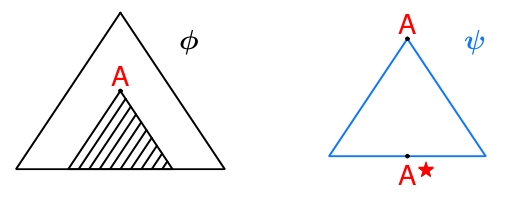
\includegraphics[scale=.4]{pics/pic2-22.jpg} & 

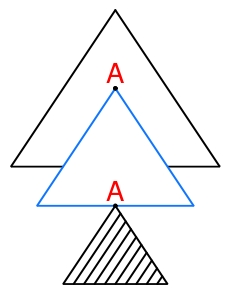
\includegraphics[scale=.35]{pics/pic2-23.jpg} \\ \hline

\multicolumn{2}{|c|}{by adjunci\'on}  \\ \hline
\end{tabular}
\end{center}\pause

\mH{Ejemplo:}\begin{tabular}{l}
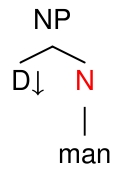
\includegraphics[scale=.45]{pics/pic2-24.jpg} \ \ \ \ \ \
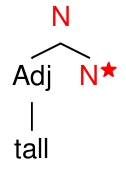
\includegraphics[scale=.45]{pics/pic2-25.jpg} \ \ \ \ \ \ 
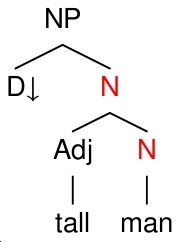
\includegraphics[scale=.45]{pics/pic2-26.jpg} 
\end{tabular}

\begin{picture}(0,0)
\put(90,40){+}
\put(155,40){$\Rightarrow$}
\end{picture}


\end{frame}


\begin{frame}
\frametitle{LTAG: TAG L\'exica} 

\begin{center}
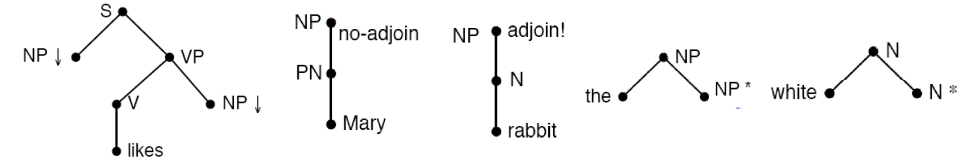
\includegraphics[scale=.4]{pics/pic3-1.jpg} \pause
\medskip

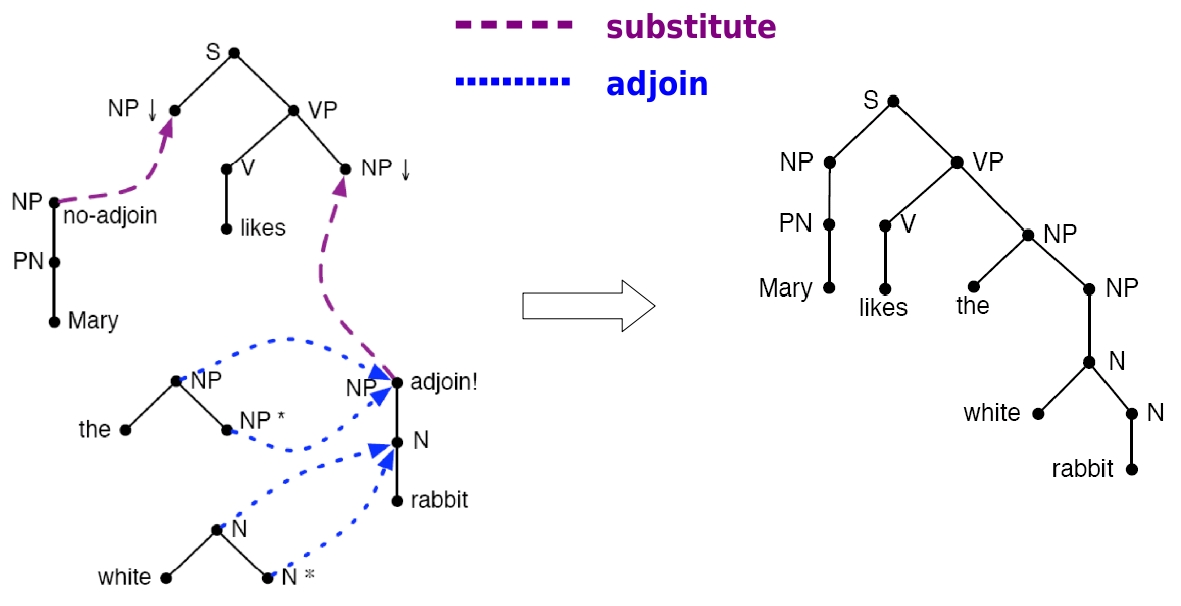
\includegraphics[scale=.3]{pics/pic3-2.jpg} 
\end{center}

\end{frame}

\begin{frame}
\frametitle{LTAG con Sem\'antica y Pragm\'atica}

\begin{center}
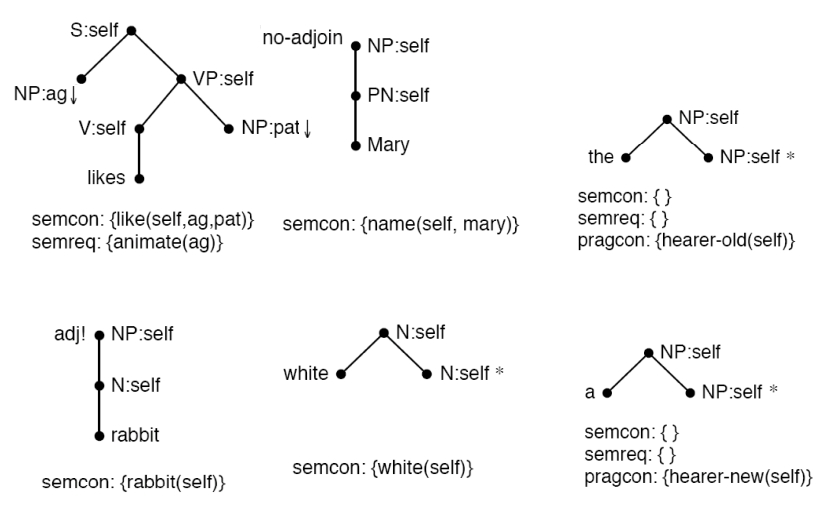
\includegraphics[scale=.4]{pics/pic3-3.jpg}
\end{center}
\end{frame}

\begin{frame}
\frametitle{Interface Sintaxis / Sem\'antica}

\begin{columns}
\column{1.2\textwidth}
\begin{itemize}
\item En una regla con informaci\'on sem\'antica como
\begin{tabular}{c}
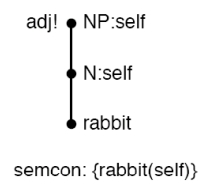
\includegraphics[scale=.4]{pics/pic3-4.jpg}
\end{tabular}

\mH{self} (y cualquier otro par\'ametro que aparezca) es una \mH{variable} que ser\'a
instanciada con cierto objeto del discurso. \pause

\item Luego de esa instanciaci\'on, con un objeto `o' digamos, la regla quedar\'a como 
\begin{tabular}{c}
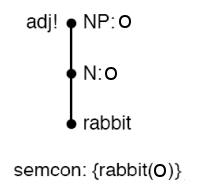
\includegraphics[scale=.4]{pics/pic3-5.jpg} \pause
\end{tabular}

\begin{picture}(0,0)
\only<3>{
\put(80,5){\begin{tikzpicture}[>=latex,inner sep=0pt,thick]
   \draw [->] (0,0) -- ++(0,.7) --++(-4,0);
  \end{tikzpicture}}}
\only<4>{
\put(83,5){\begin{tikzpicture}[>=latex,inner sep=0pt,thick]
   \draw [->] (0,0) -- ++(0,1.8) --++(-8.5,0);
  \end{tikzpicture}}}
\only<5>{
\put(90,-27){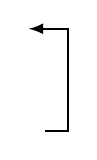
\begin{tikzpicture}[>=latex,inner sep=0pt,thick]
   \draw [->] (0,0) --(.3,0) -- ++(0,1.3) --++(-.5,0);
  \end{tikzpicture}}}
\end{picture}
\vspace*{-.5cm}

\item Podemos pensar que cuando la palabra `rabbit' es usada,\pause\ un referente $o$ al 
objeto nombrado es introducido,\pause\ junto con la asserci\'on sem\'antica del predicado rabbit(o) 

\end{itemize}
\end{columns}
\end{frame}

\begin{frame}
\frametitle{Surface Realization}

\begin{itemize}
\item Tenemos ahora todas las herramientas como para definir un algoritmo de \mH{surface realization}. 

\item Recordemos que antes de llegar a esta etapa, habiamos llegado a una \mH{especificaci\'on a nivel de
frases} de cada sentencia que quer\'iamos generar. 

\item Si el objetivo es usar LTAG para surface realization, deber\'iamos contar, en el momento de generar 
cada sentencia con
\begin{itemize}
\item la \mH{sem\'antica} que queremos generar 
\item enriquecida quiz\'as con \mH{informaci\'on del dominio} (background knowledge)   
\item informaci\'in sobre \mH{el contexto} generado y a generar (e.g., qu\'e elementos ya han sido introducidos)
\end{itemize}

\end{itemize}
\end{frame}

\begin{frame}
\frametitle{Surface Realization: The White Rabbit}

\begin{itemize}
\item Suppongamos que queremos generar una frase correspondiente a la sem\'antica 
\medskip

\centerline{\{rabbit(r), white(r)\}} 
\medskip

sabiendo que r ya ha sido mencionada anteriormente 
\medskip

\centerline{ hearer-old(r)}

\item Busquemos en nuestra gram\'atica, los \'arboles que podr\'ian \mH{contribuir a la generaci\'on} 

\begin{picture}(0,80)
\only<2>{
\put(30,10){
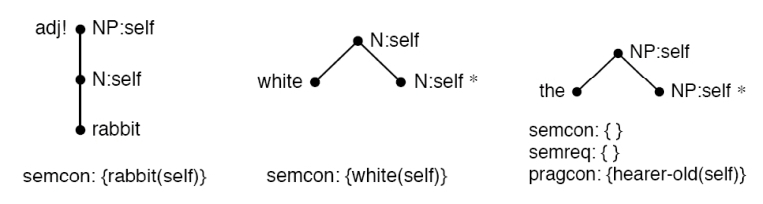
\includegraphics[scale=.4]{pics/pic3-8.jpg}}}
\only<3>{
\put(30,10){
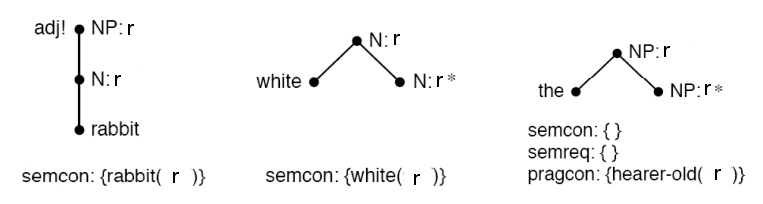
\includegraphics[scale=.4]{pics/pic3-9.jpg}}}
\end{picture} 
 
\end{itemize}

\end{frame}

\begin{frame}
\frametitle{Surface Realization}

\mH{Para comunicar}: \{ like(e,m,r), name(m,mary), rabbit(r), white(r) \}\\
\mH{Contexto de discurso}: \{hearer-old(r)\}\\
\mH{Conicimiento de dominio}: \{animate(r)\}

\begin{picture}(0,150)
\only<2>{
\put(50,0){
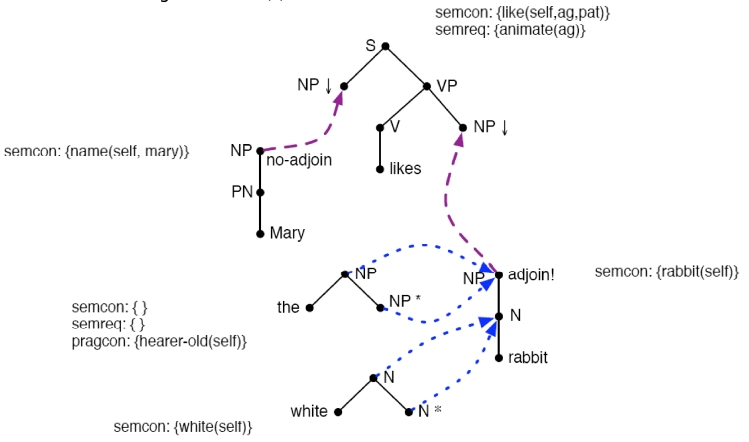
\includegraphics[scale=.4]{pics/pic3-6.jpg}
}}
\only<3>{
\put(50,0){
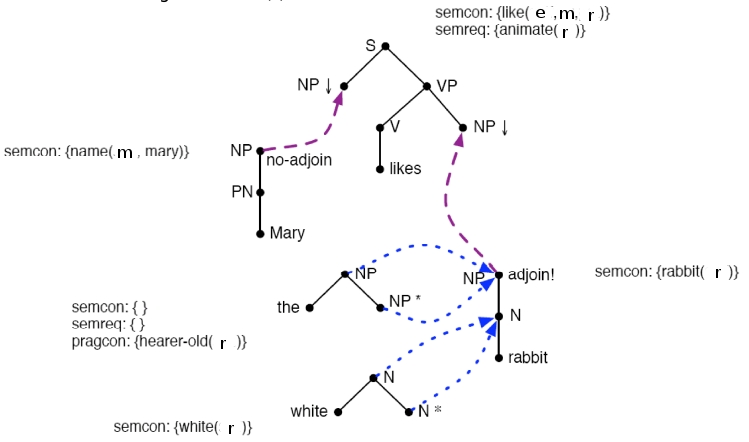
\includegraphics[scale=.4]{pics/pic3-7.jpg}
}}
\end{picture}
\end{frame}

\begin{frame}
\frametitle{El Algoritmo de Realizaci\'on}

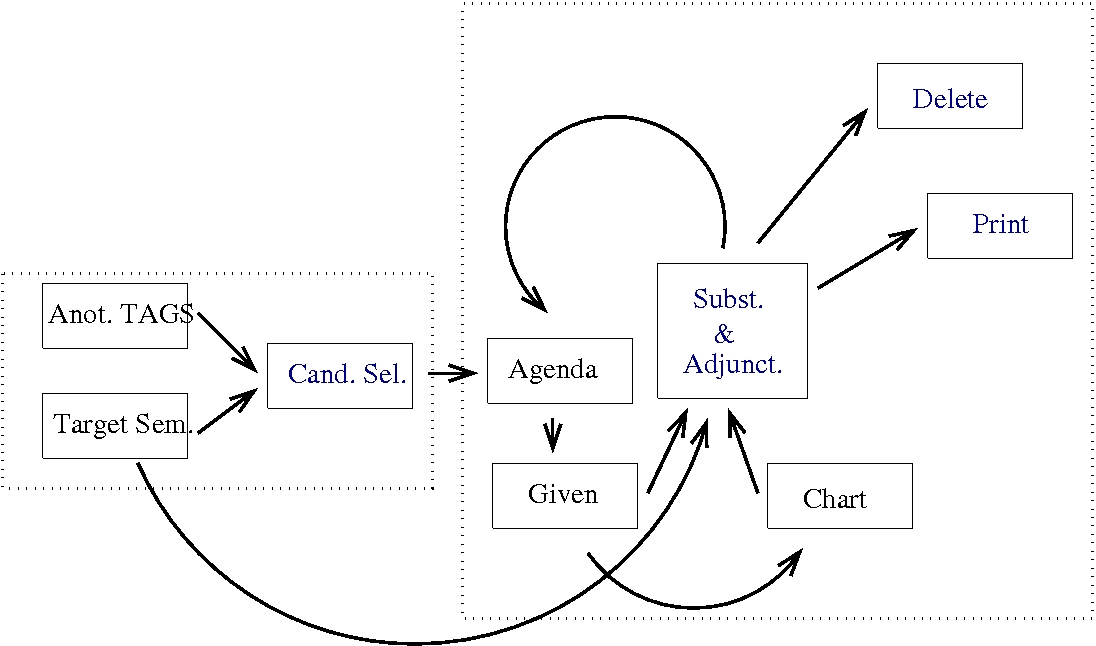
\includegraphics[scale=.3]{pics/gen.jpg}

\end{frame}

\begin{frame}
\frametitle{Surface Realization}

\begin{itemize}
\item El problema de realizacion para una TAG arbitraria es \mH{NP-complete}

\item Podemos tratar de definir una gram\'atica con buenas propiedades para 
disminuir la complejidad
\begin{itemize}
\item Si nos arboles auxiliares \mH{no tienen nodos de sustituci\'on}
\item Podemos aplicar primero \mH{todas} las operaciones de sustitucion
\item Y s\'olo despues hacer adjunci\'on para completar la sem\'antica target
\end{itemize}

\item Existen diferentes heur\'isticas para la eleccion de \mH{given}

\end{itemize}

\end{frame}

\begin{frame}
\frametitle{Temas de Investigaci\'on}

\begin{itemize}
\item Si la gram\'atica es grande pueden existir muchas formas de realizar una 
misma sem\'antica.  El algoritmo que vimos no incluye ninguna heur\'istica para 
elegir `la mejor' representaci\'on. 
\begin{itemize}
\item Podriamos generar todas las opciones y luego producir un ranking. 
\item Ser\'ia m\'as eficiente si podemos generar s\'olo la m\'as alta en el ranking.
\end{itemize}

\item Si la gram\'atica es grande, producirla y mantenerla es extremadamente 
costoso. 
\begin{itemize}
\item Podemos generar una meta-gram\'atica que genere la gram\'atica
\end{itemize}

\item Cu\'al es el mejor lenguaje para representar la sem\'antica? 

\item Como afecta los `agregados a TAG' a si poder expresivo?
\end{itemize}
\end{frame}


\begin{frame}
\frametitle{Lo que Vemos Hoy}

\begin{itemize}
\item \mH{TAGs y Surface Realization}
\item Generaci\'on de Expresiones Referenciales
\end{itemize}
\end{frame}

\begin{frame}
\frametitle{Lo que Vemos Hoy}

\begin{itemize}
\item TAGs y Surface Realization
\item \mH{Generaci\'on de RE}
\begin{tabular}{|l}
Expresiones Referenciales\\
Escala de Familiaridad\\
Generaci\'on de Definite NPs\\
ER Relacionales 
\end{tabular}
\end{itemize}
\end{frame}

\begin{frame}
\frametitle{Generando Expresiones Referenciales}

\begin{quote}

\textbf{He claims record}\medskip

The 22-year-old computer science undergraduate from Bath is
claiming a world record for the longest distance ridden on a
unicycle in 24 hours.\medskip

A unicycling student covered exactly 282 miles at Aberystwy
University's athletics track.\medskip

Sam Wakeling was aiming to beat the existing record of 235.3
miles.
\end{quote}

\end{frame}

\begin{frame}
\frametitle{Generando Expresiones Referenciales}

\begin{quote}

\textbf{\mH{He} claims record}\medskip

\mH{The 22-year-old computer science undergraduate from Bath} is
claiming a world record for the longest distance ridden on a
unicycle in 24 hours.\medskip

\mH{A unicycling student} covered exactly 282 miles at Aberystwy
University's athletics track.\medskip

\mH{Sam Wakeling} was aiming to beat the existing record of 235.3
miles.
\end{quote}

\end{frame}

\begin{frame}
\frametitle{Generando Expresiones Referenciales}

\begin{quote}
\textbf{\mH{Unicycling student} claims record}\medskip

\mH{A student} is claiming a world record for the longest distance ridden
on a unicycle in 24 hours.\medskip

\mH{Sam Wakeling} covered exactly 282 miles at Aberystwyth
University's athletics track.\medskip

\mH{The 22-year-old computer science undergraduate from Bath} was
aiming to beat the existing record of 235.3 miles.
\end{quote}

\end{frame}

\begin{frame}
\frametitle{Terminolog\'ia}

\begin{itemize}
\item \mH{Expresi\'on Referencial:}
Una expresi\'on ling\"u\'istica (t\'ipicamente un NP) que el speaker
usa para identificar una entidad (en el discurso)

\item \mH{Referente:}
La entidad a la que el speker refiere mediante la expresion referencial

\item \mH{Referencia:}
El proceso de identificar la entidad usando la expresi\'on referencial

\end{itemize}
\end{frame}


\begin{frame}
\frametitle{Referencia y Discurso}

Una entidad dada puede ser referenciada de muchas maneras diferentes

\begin{enumerate}
\item 
Noam Chomsky has given a talk today.

\item
One of the people working at MIT has given a talk today.

\item 
A person who is working at MIT has given a talk today.

\item 
A person has given a talk today.
\end{enumerate}
\end{frame}

\begin{frame}
\frametitle{Referencia y Discurso}

\mH{Referencia y forma ling\"u\'istica}
\medskip

La forma ling\"u\'istica de una expresion referencial \mH{refleja el
estado actual del referente en el discurso} (m\'as exactamente, 
las creencias del speaker sobre el modelo del discurso del hearer). 
\medskip
\pause

Usualmente:

\begin{itemize}
\item referentes nuevos en el discurso se introducen mediante indefinite NPs: \mH{a cat}

\item referentes ya existentes en el discurso son referidos mediante definite NPs y pronombres:
\mH{the cat} / \mH{it}
\end{itemize}
\end{frame}

\begin{frame}
\frametitle{Lo que Vemos Hoy}

\begin{itemize}
\item TAGs y Surface Realization
\item \mH{Generaci\'on de RE}
\begin{tabular}{|l}
Expresiones Referenciales\\
\mH{Escala de Familiaridad}\\
Generaci\'on de Definite NPs\\
ER Relacionales 
\end{tabular}
\end{itemize}
\end{frame}


\begin{frame}
\frametitle{Prince (1981, 1992): Forma Ling\"u\'istica  \& Escala de Familiaridad}

\mH{Escalas de Familiaridad:}
\medskip

\begin{itemize}
\item \mH{Desde el punto de vista del speaker/writer:}
Qu\'e hip\'otesis sobre el hearer/reader influencian la elecci\'on de una expresi\'on 
referencial?

\item \mH{Desde el punto de vista del hearer/reader:}
Qu\'e conclusion sacar\'a de la elecci\'on hecha de una determinada expresi\'on 
referencial?
\end{itemize}

\end{frame}

\begin{frame}
\frametitle{Dimensiones de Familiaridad (Prince 1981, 1992)} \small

\begin{columns}
\column{1.1\textwidth}
\begin{center}
\begin{tabular}{|p{4cm}|l|l|} \hline
status of the referent\newline
(assumed by the speaker)

& discourse-new

& discourse-old\\ \hline

hearer-new & \only<2>{\mH{brand-new}}\only<3->{brand-new} & \only<3>{\mH{---}}\only<4->{---} \\ \hline

hearer-old & \only<4>{\mH{unusued}}\only<5->{unusued} & \only<5>{\mH{evoked}}\only<6->{evoked} \\ \hline 
\end{tabular}
\end{center}
\pause

\vspace*{-.5cm}
\begin{itemize}
\item \mH{brand-new}: introducci\'on de un nuevo referente en el discurso 
representando una entidad desconocida: \mH{a student}\pause\pause
\vspace*{-.2cm}

\item \mH{unused}: introducci\'on de un nuevo referente en el discurso 
representando una entidad conocida: \mH{Queen Elisabeth}\pause
\vspace*{-.2cm}

\item \mH{evoked}: una entidad relacionada con otra que
\vspace*{-.3cm}

\begin{itemize}
\item has sido referida antes (en el discurso)\\
\mH{The 22-year old computer science undergraduate from Bath}

\item est\'a presente: \mH{you} \pause
\end{itemize}
\vspace*{-.4cm}

\item \mH{inferrable}: introducci\'on de un nuevo referente en el discurso
cuya relaci\'on a una entidad conocida es irreferible (es hearer-old pero 
no es ni discourse-new ni discourse-old)\\

Peter walked towards the house. \mH{The door} was open.
\end{itemize}

\end{columns}
\end{frame}

\begin{frame}
\frametitle{Escala de Familiaridad de Prince}

\begin{picture}(0,0)
\only<1>{\put(-20,-130){
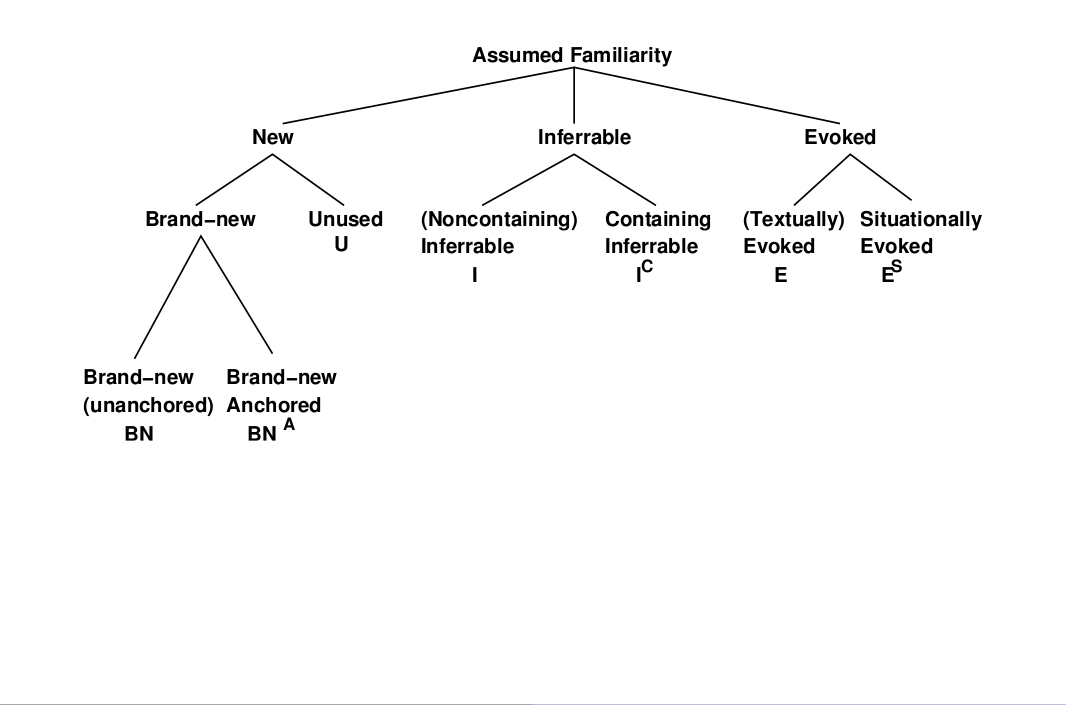
\includegraphics[scale=.4]{pics/pic3-10.jpg}}}
\only<2>{\put(-20,-130){
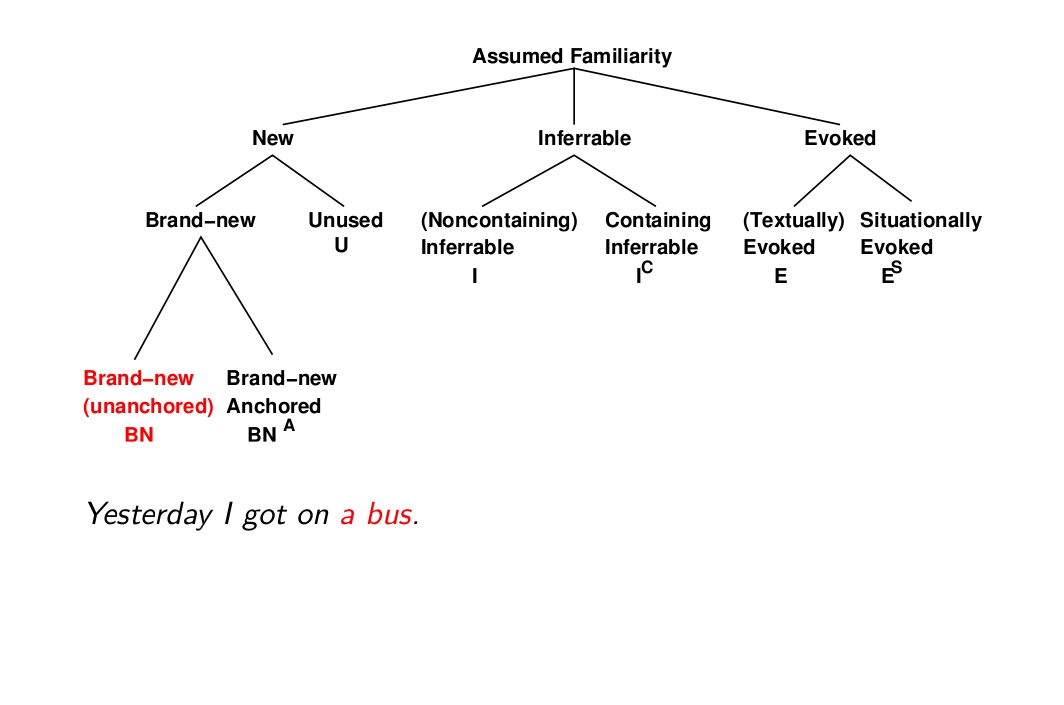
\includegraphics[scale=.4]{pics/pic3-11.jpg}}}
\only<3>{\put(-20,-130){
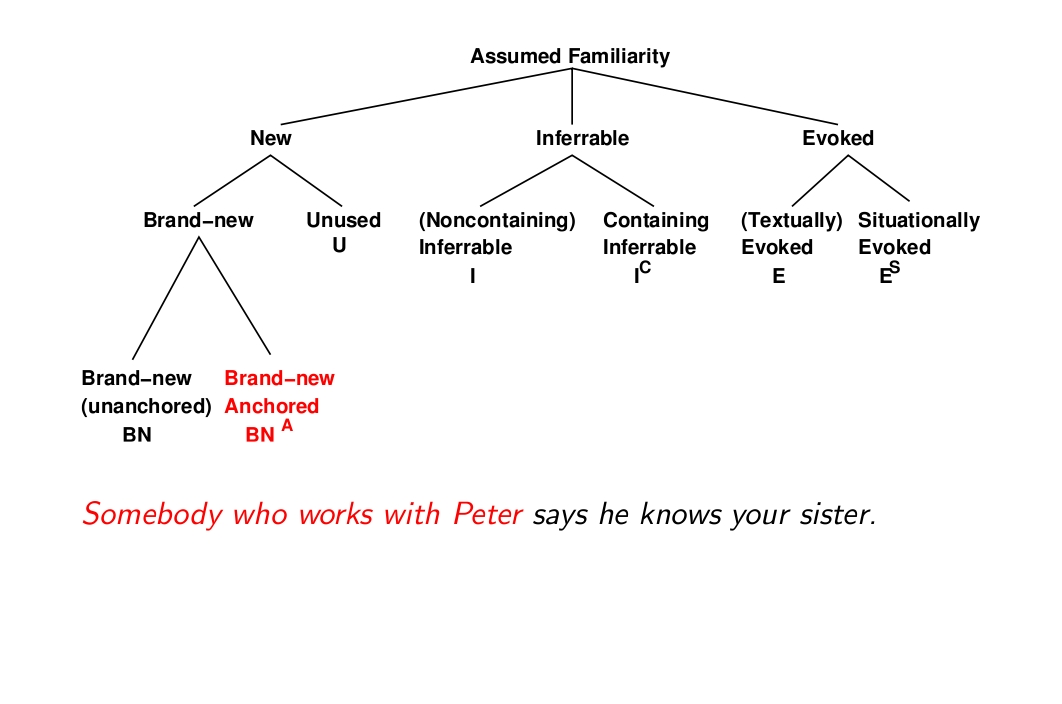
\includegraphics[scale=.4]{pics/pic3-12.jpg}}}
\only<4>{\put(-20,-130){
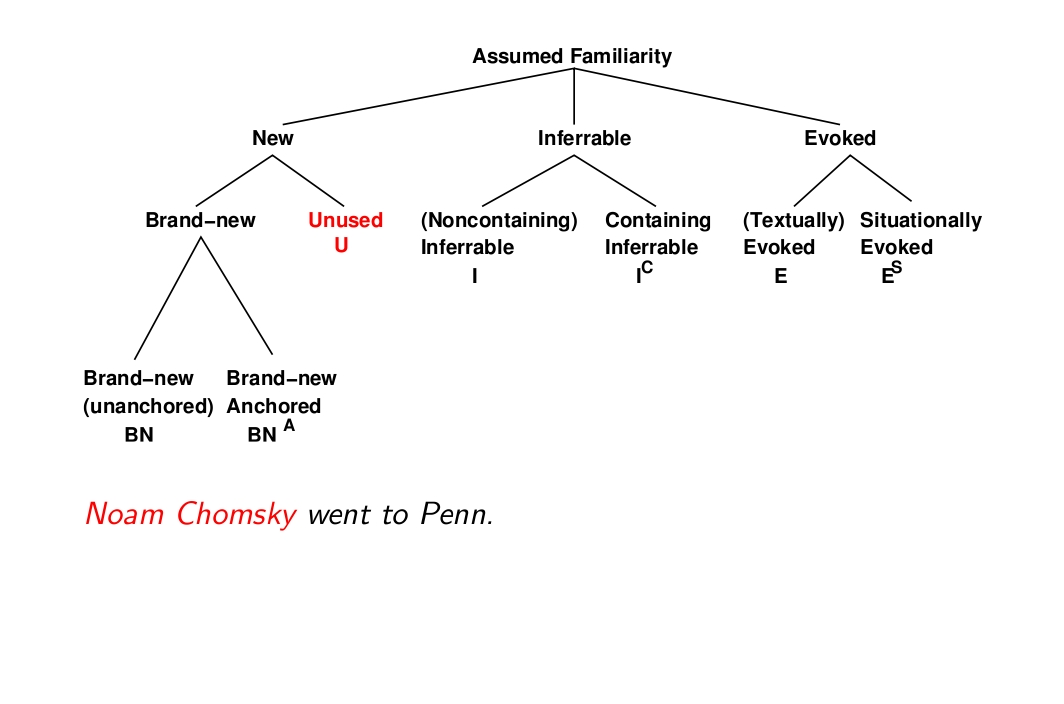
\includegraphics[scale=.4]{pics/pic3-13.jpg}}}
\only<5>{\put(-20,-130){
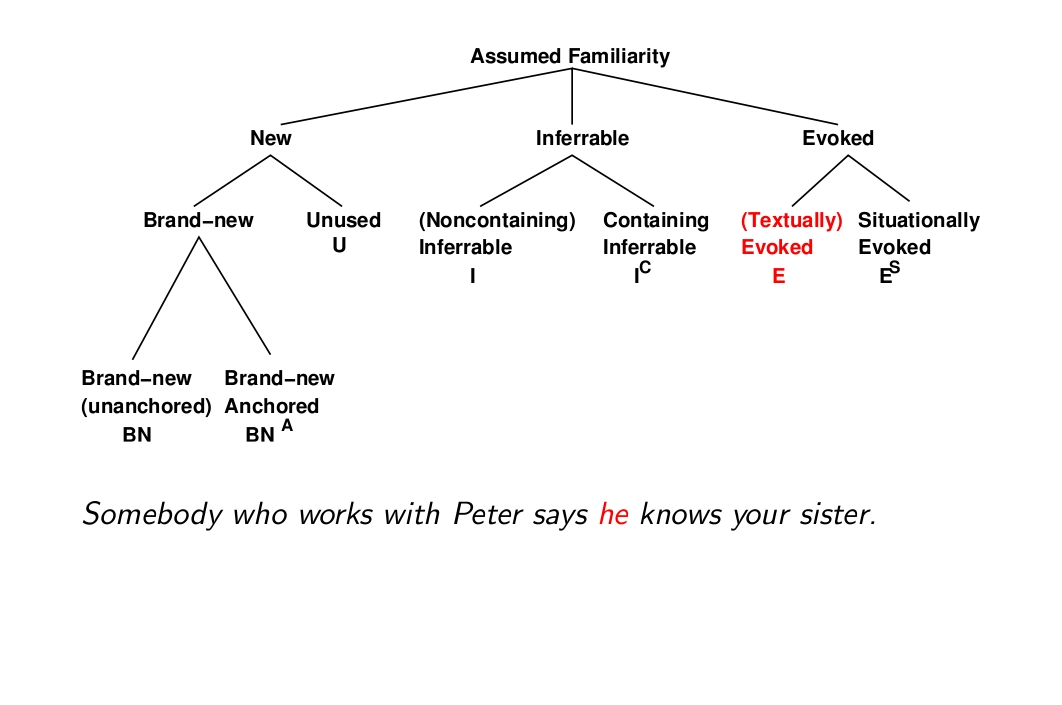
\includegraphics[scale=.4]{pics/pic3-14.jpg}}}
\only<6>{\put(-20,-130){
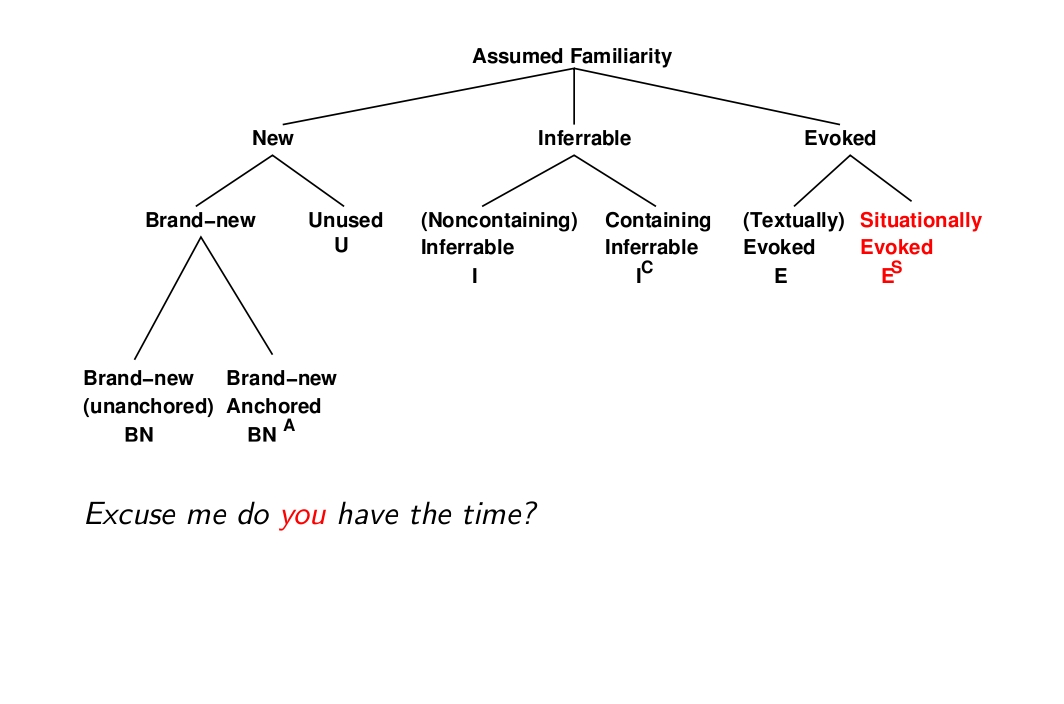
\includegraphics[scale=.4]{pics/pic3-15.jpg}}}
\only<7>{\put(-20,-130){
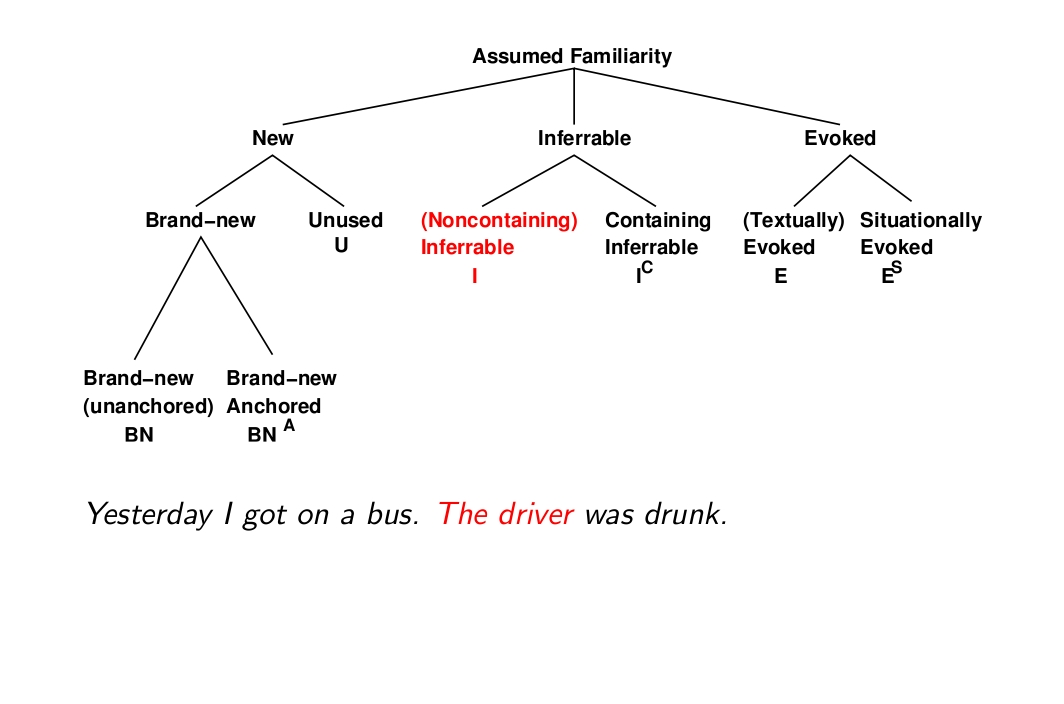
\includegraphics[scale=.4]{pics/pic3-16.jpg}}}
\only<8>{\put(-20,-130){
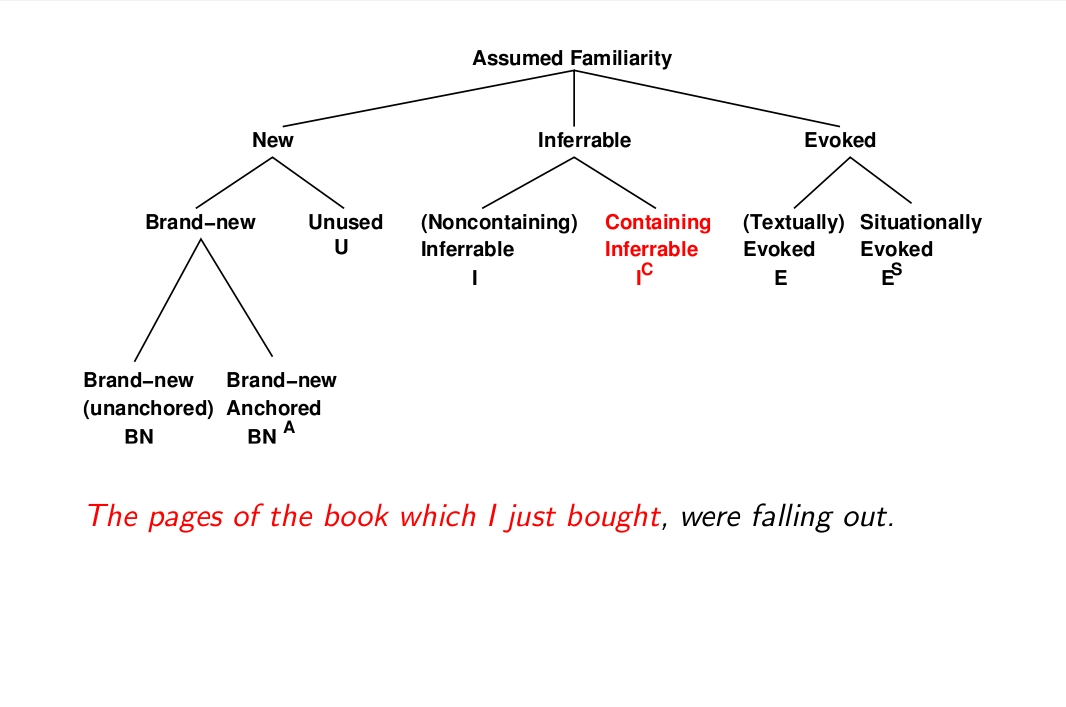
\includegraphics[scale=.4]{pics/pic3-17.jpg}}}
\only<8>{\put(-20,-130){
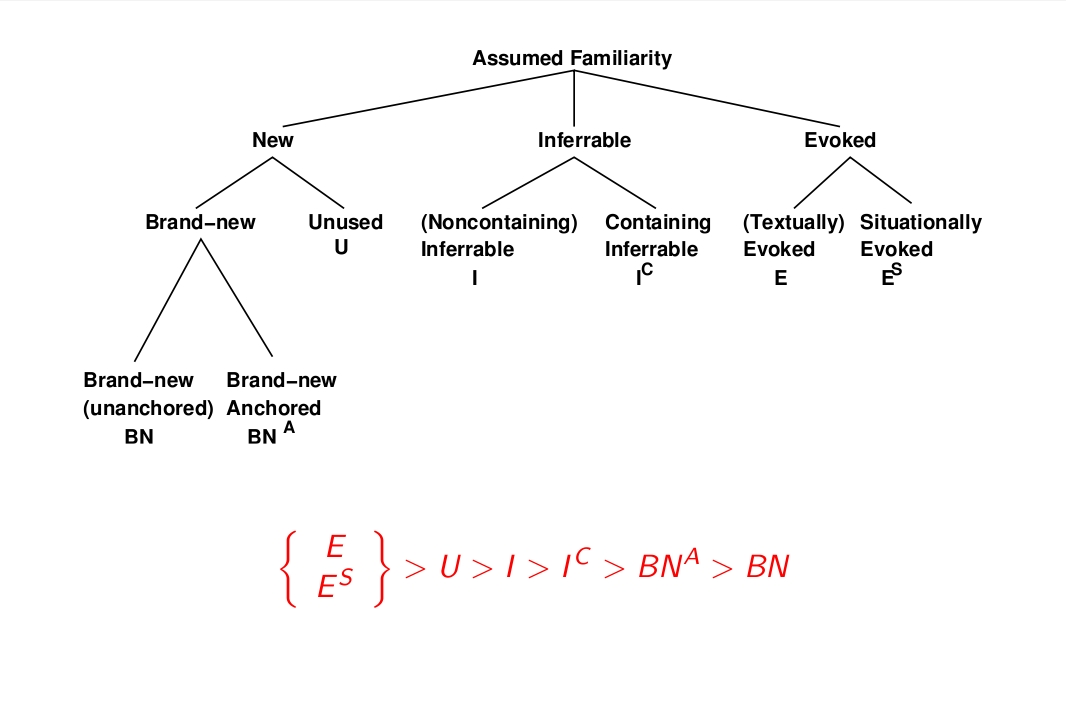
\includegraphics[scale=.4]{pics/pic3-18.jpg}}}
\end{picture}
\end{frame}

\begin{frame}
\frametitle{Escala de Familiaridad de Prince}

\begin{center}
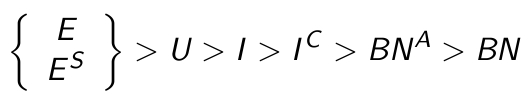
\includegraphics[scale=.4]{pics/pic3-19.jpg}
\end{center}

\begin{enumerate}
\item Noam Chomsky has given a talk today. ($U$)

\item One of the people working at MIT has given a talk today. ($I^C$)

\item A person who is working at MIT has given a talk today.
($BN^A$)

\item A person has given a talk today. ($BN$)
\end{enumerate}

\end{frame}

\begin{frame}
\frametitle{Lo que Vemos Hoy}

\begin{itemize}
\item TAGs y Surface Realization
\item \mH{Generaci\'on de RE}
\begin{tabular}{|l}
Expresiones Referenciales\\
Escala de Familiaridad\\
\mH{Generaci\'on de Definite NPs}\\
ER Relacionales 
\end{tabular}
\end{itemize}
\end{frame}

\begin{frame}
\frametitle{Generando Expresiones Referenciales: Ejemplo}

\begin{center}
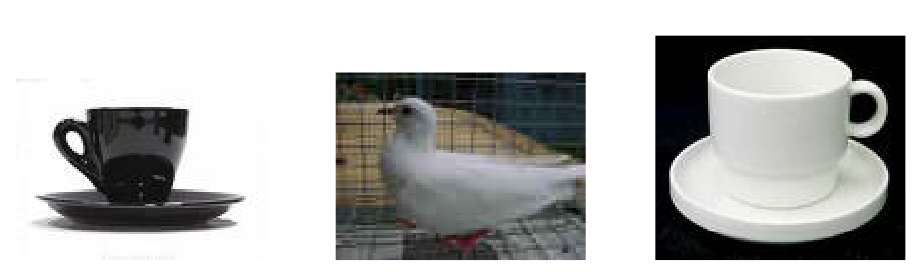
\includegraphics[scale=.45]{pics/pic3-20.jpg}
\end{center}

\end{frame}

\begin{frame}
\frametitle{Caso Concreto}

\vspace*{-.5cm}
\begin{center}
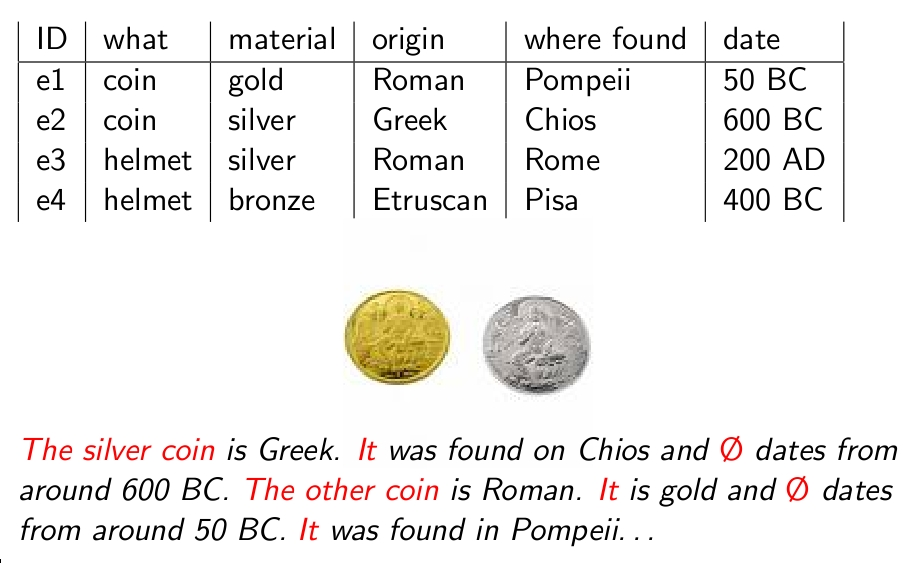
\includegraphics[scale=.45]{pics/pic3-21.jpg}
\end{center}

\end{frame}

\begin{frame}
\frametitle{Generaci\'on de definite NPs}

Tomemos en cuenta las M\'aximas de Grice:

\begin{itemize}

\item \mT{Quality}\\
Say the truth.

\item \mT{Quantity}\\
\only<1>{Be as informative as possible.}
\only<2->{\mH{Be as informative as possible.}}

\item \mT{Relevance}\\
Be relevant.

\item \mT{Manner}\\
\only<1>{Be brief.}\only<2->{\mH{Be brief.}} Avoid ambiguity. Be orderly.\pause\pause

\end{itemize}

$\Rightarrow$ Elegir la RE \mH{m\'as corta} que \mH{discrimita} a
la entidad target de todas las demas entidades del modelo de discurso 
(los distractores). 

\end{frame}

\begin{frame}
\frametitle{Generaci\'on de Definite NPs}

\mH{Estrategia:}
Las entidades del discurso estan descriptas en terminos de distintos valores
de sus atributos (atribute-value pairs, AVPs)

$\Rightarrow$ realizar el conjunto mas peque\~no de valores que identifica
un\'ivocamente a la entidad \pause

\begin{picture}(0,80)
\only<2>{\put(30,0){
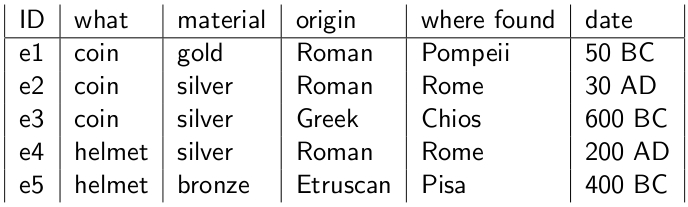
\includegraphics[scale=.5]{pics/pic3-22.jpg}}}
\only<3->{\put(30,0){
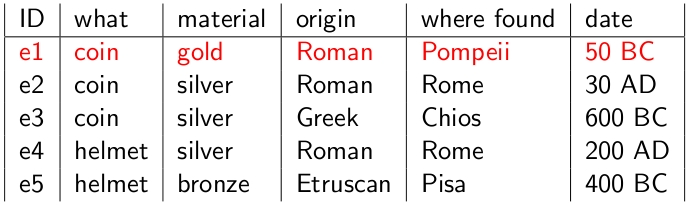
\includegraphics[scale=.5]{pics/pic3-23.jpg}}}
\end{picture}\pause \pause

\mH{Good}: \ 
\begin{tabular}{|l}
the gold coin (the golden one, the object made of gold)\\
the coin found in Pompeii\\
the coin dating from 50 BC\\
\end{tabular}\pause

\mH{No Good}: \
\begin{tabular}{|l}
the gold coin found in Pompeii (demasiado inform.)\\
the Roman coin (no un\'ivoca)
\end{tabular}
\end{frame}

\begin{frame}
\frametitle{Generaci\'on de Definite NPs}

\mH{Estrategia de B\'usqueda:} computar el poder discriminatorio de 
cada AVP y elegir el m\'as alto hasta que la entidad target es 
un\'ivoca.
\medskip

\mH{Distractores}: $U = \{x_1, x_2, \ldots, x_n\}$
\medskip

\mH{Poder discriminatorio de un AVP del objeto target dado U}:
$$
F(\langle a,v \rangle, U) = \frac{n-k}{n}
$$

donde $k$ es el n\'umero de distractores para el que $\tup{a,v}$ es cierto.
\end{frame}

\begin{frame}
\frametitle{Generaci\'on de Definite NPs: Ejemplo}

\begin{center}
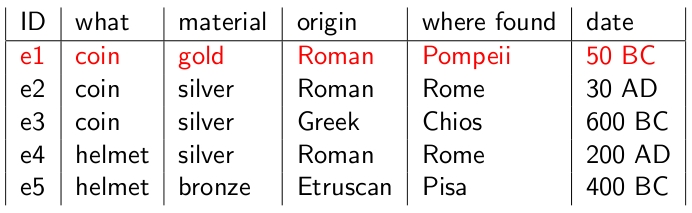
\includegraphics[scale=.5]{pics/pic3-24.jpg}
\end{center}

\vspace*{-.5cm}
$$
F(\langle material,gold \rangle,U) = \frac{4-0}{4} = 1 \pause
$$
\vspace*{-.1cm}
$$
F(\langle origin,Roman \rangle,U) = \frac{4-2}{4} = 0.5 \pause
$$

Como elegimos entre AVPs con el mismo \'indice? Usualmente asumimos 
que los atributos estan ordenados a priori
$$
material > origen > where found > \ldots
$$

\end{frame}

\begin{frame}
\frametitle{Lo que Vemos Hoy}

\begin{itemize}
\item TAGs y Surface Realization
\item \mH{Generaci\'on de RE}
\begin{tabular}{|l}
Expresiones Referenciales\\
Escala de Familiaridad\\
\mH{Generaci\'on de Definite NPs}\\
ER Relacionales 
\end{tabular}
\end{itemize}
\end{frame}


\begin{frame}
\frametitle{Expresiones Referenciales Relacionales}

\begin{itemize}
\item Sabemos entonces como referirnos a elementos del dominio del discurso \pause

\item Practiquemos:
\begin{picture}(0,0)
\only<2>{\put(102,-88){
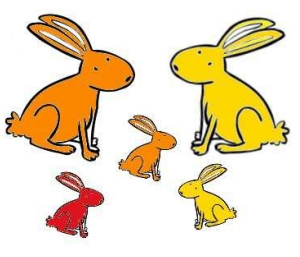
\includegraphics[scale=.4]{pics/pica-1.jpg}}}
\end{picture}\pause

\item Ahora probemos con este dominio:

\begin{picture}(0,0)
\only<3>{\put(102,-88){

\includegraphics[scale=.4]{pics/pica-2.jpg}}}
\end{picture}

\end{itemize}

\vspace*{3cm}

\end{frame}

\begin{frame}
\frametitle{Infinite Recursion}

\begin{itemize}

\item Los algoritmos originalmente propuestos para computar expresiones referenciales 
intentaban \mH{reusar} el algoritmo que vimos:

\begin{itemize}
\item Mantenemos un \mH{stack} the objetos a describir
\item Describimos el objeto en el \mH{tope} del stack
\item Cuando utilizamos una una relaci\'on en la descripci\'on ponemos el nuevo indiv\'iduo 
en el stack. 
\item Cuando completamos la descripcion de un objeto lo sacamos del stack\pause

\end{itemize}

\item Este algoritmo corre el riesgo de caer en una regresi\'on infinita
\begin{quote}
the rabbit in the hat with the rabbit in the hat with the rabbit \ldots
\end{quote}
\end{itemize}

\end{frame}

\begin{frame}
\frametitle{Modelos y F\'ormulas}

\begin{center}
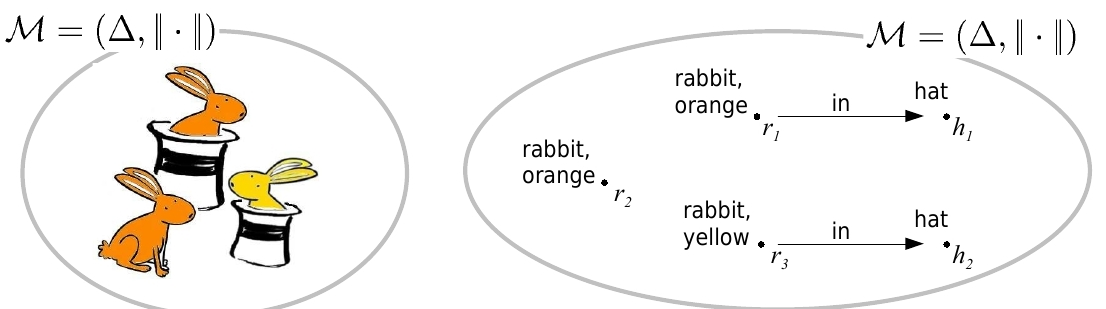
\includegraphics[scale=.25]{pics/modelo1.jpg}
\end{center}\pause

\begin{center}
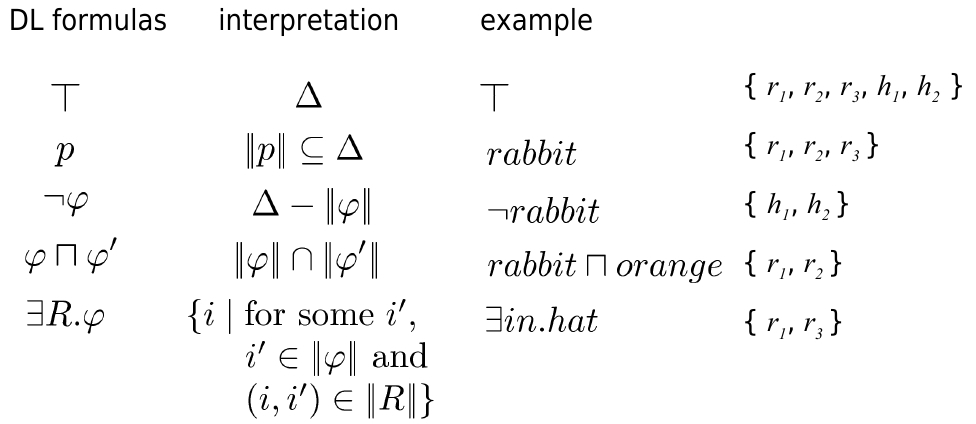
\includegraphics[scale=.25]{pics/modelo2.jpg}
\end{center}

\end{frame}


\begin{frame}
\frametitle{Expresiones Referenciales Relacionales}
\begin{picture}(0,0)
\put(160,-70){
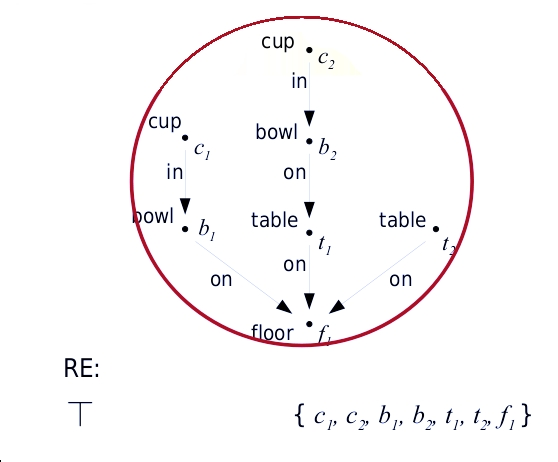
\includegraphics[scale=.4]{pics/pic4-1.jpg}}
\end{picture}


\begin{columns}
\column{6.5cm}
\begin{itemize}
\item \mH{Conenzamos con un conjunto conteniendo todos los elementos}
\end{itemize}
\column{5cm}
\end{columns}

\end{frame}


\begin{frame}
\frametitle{Expresiones Referenciales Relacionales}
\begin{picture}(0,0)
\put(172,-100){
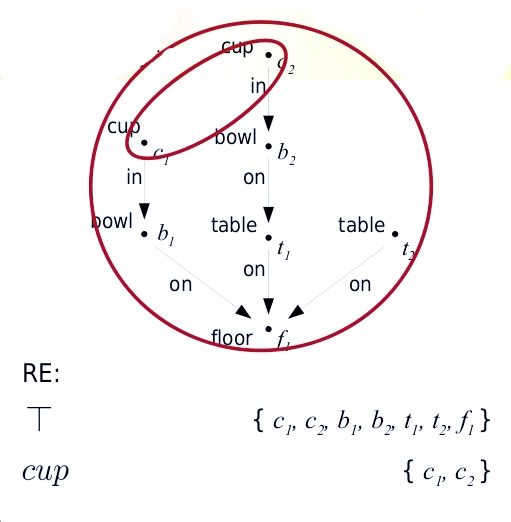
\includegraphics[scale=.4]{pics/pic4-2.jpg}}
\end{picture}

\begin{columns}
\column{6.5cm}
\begin{itemize}
\item Conenzamos con un conjunto conteniendo todos los elementos
\item \mH{Cada propiedad identifica un conjunto de elementos}
\end{itemize}
\column{5cm}
\end{columns}

\end{frame}

\begin{frame}
\frametitle{Expresiones Referenciales Relacionales}
\begin{picture}(0,0)
\put(175,-115){
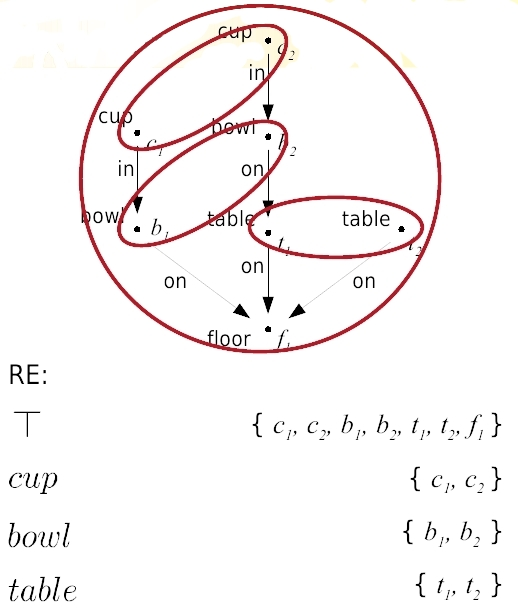
\includegraphics[scale=.27]{pics/picx3.jpg}}
\end{picture}


\begin{columns}
\column{6.5cm}
\begin{itemize}
\item Conenzamos con un conjunto conteniendo todos los elementos
\item Cada propiedad identifica un conjunto de elementos
\end{itemize}
\column{5cm}
\end{columns}

\end{frame}

\begin{frame}
\frametitle{Expresiones Referenciales Relacionales}
\begin{picture}(0,0)
\put(175,-145){
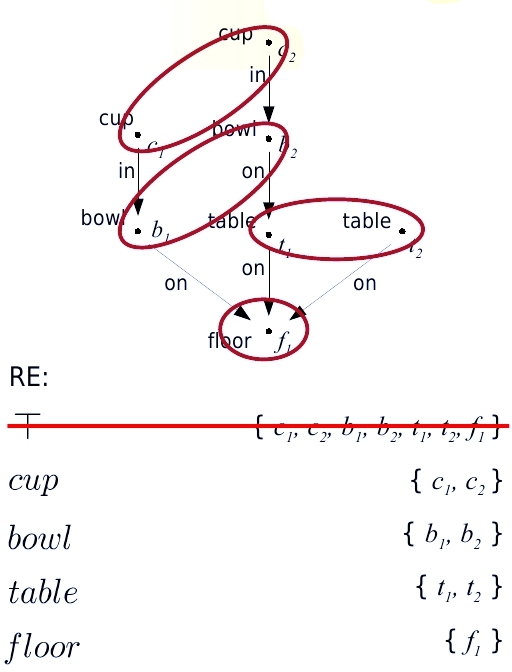
\includegraphics[scale=.27]{pics/picx4.jpg}}
\end{picture}


\begin{columns}
\column{6.5cm}
\begin{itemize}
\item Conenzamos con un conjunto conteniendo todos los elementos
\item Cada propiedad identifica un conjunto de elementos
\item \mH{Cuando un conjunto de particiones cubre totalmente otra, podemos eliminarla}
\end{itemize}
\column{5cm}
\end{columns}

\end{frame}

\begin{frame}
\frametitle{Expresiones Referenciales Relacionales}
\begin{picture}(0,0)
\put(175,-160){
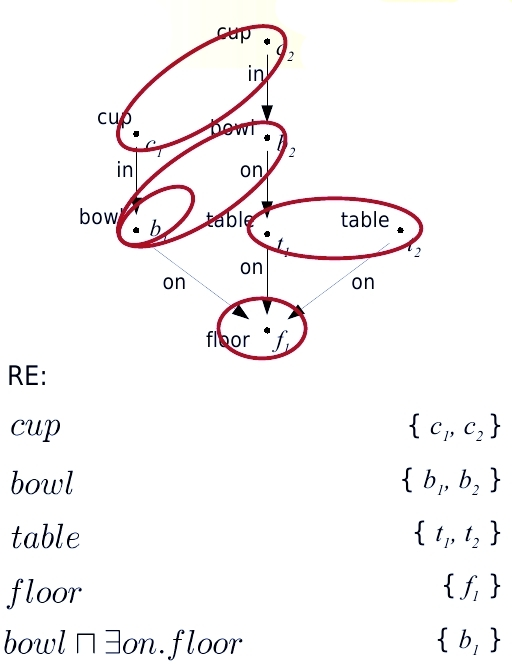
\includegraphics[scale=.27]{pics/picx5.jpg}}
\end{picture}


\begin{columns}
\column{6.5cm}
\begin{itemize}
\item Conenzamos con un conjunto conteniendo todos los elementos
\item Cada propiedad identifica un conjunto de elementos
\item Cuando un conjunto de particiones cubre totalmente otra, podemos eliminarla
\item \mH{Al terminar con las propiedades, hacemos regresion sobre las relaciones.} 
\end{itemize}
\column{5cm}
\end{columns}

\end{frame}

\begin{frame}
\frametitle{Expresiones Referenciales Relacionales}
\begin{picture}(0,0)
\put(173,-175){
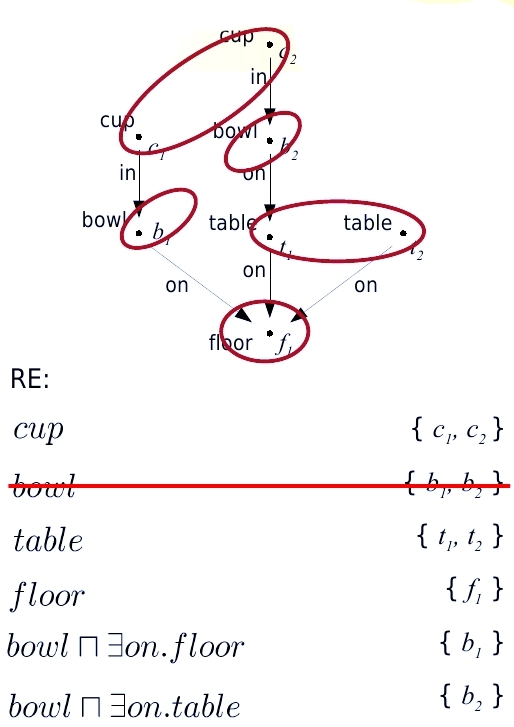
\includegraphics[scale=.27]{pics/picx6.jpg}}
\end{picture}

\begin{columns}
\column{6.5cm}
\begin{itemize}
\item Conenzamos con un conjunto conteniendo todos los elementos
\item Cada propiedad identifica un conjunto de elementos
\item Cuando un conjunto de particiones cubre totalmente otra, podemos eliminarla
\item Al terminar con las propiedades, hacemos regresion sobre las relaciones 
\end{itemize}
\column{5cm}
\end{columns}

\end{frame}

\begin{frame}
\frametitle{Expresiones Referenciales Relacionales}
\begin{picture}(0,0)
\put(173,-175){
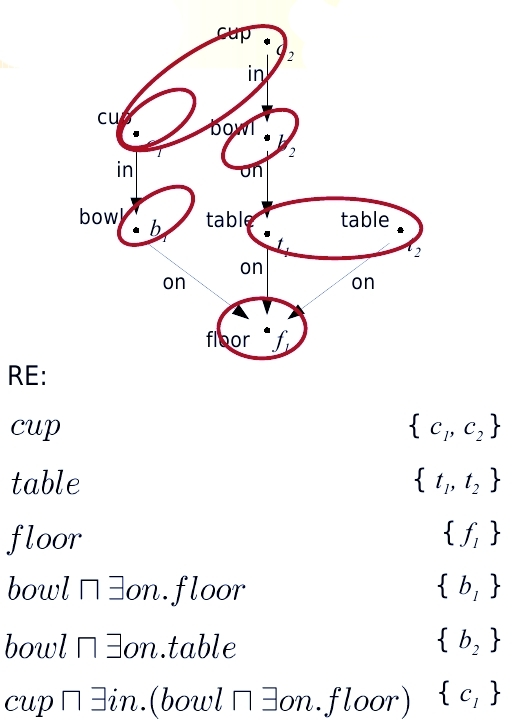
\includegraphics[scale=.27]{pics/picx7.jpg}}
\end{picture}

\begin{columns}
\column{6.5cm}
\begin{itemize}
\item Conenzamos con un conjunto conteniendo todos los elementos
\item Cada propiedad identifica un conjunto de elementos
\item Cuando un conjunto de particiones cubre totalmente otra, podemos eliminarla
\item Al terminar con las propiedades, hacemos regresion sobre las relaciones 
\end{itemize}
\column{5cm}
\end{columns}
\end{frame}

\begin{frame}
\frametitle{Expresiones Referenciales Relacionales}
\begin{picture}(0,0)
\put(173,-180){
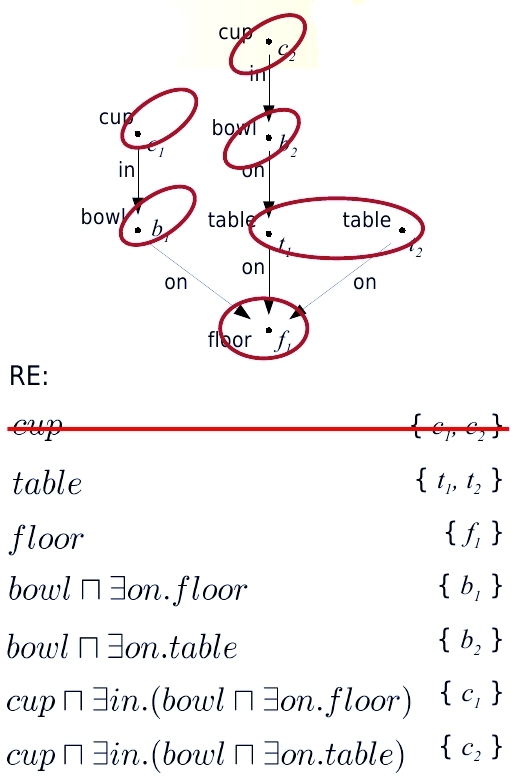
\includegraphics[scale=.27]{pics/picx8.jpg}}
\end{picture}

\begin{columns}
\column{6.5cm}
\begin{itemize}
\item Conenzamos con un conjunto conteniendo todos los elementos
\item Cada propiedad identifica un conjunto de elementos
\item Cuando un conjunto de particiones cubre totalmente otra, podemos eliminarla
\item Al terminar con las propiedades, hacemos regresion sobre las relaciones 
\end{itemize}
\column{5cm}
\end{columns}
\end{frame}

\begin{frame}
\frametitle{Caracter\'isticas del Algoritmo}

\begin{itemize}

\item Todas las REs se computan en paralelo

\item El algoritmo es muy eficiente
\begin{picture}(0,0)
\put(0,-120){
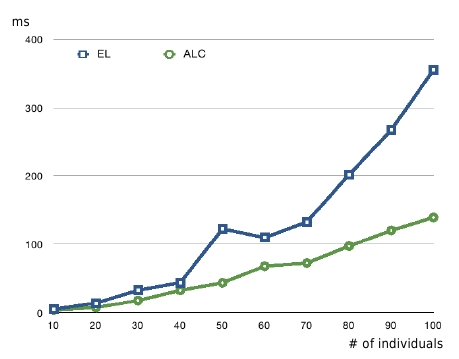
\includegraphics[scale=.35]{pics/graph.jpg}}
\end{picture}


\item Si el modelo cambia, pueden \\ recomputarse solamente 
los\\ cambios necesarios. 

\item Est\'a basado en la noci\'on de\\ simulaci\'on entre 
elementos de\\ un modelo
\end{itemize}
\end{frame}



\end{document}
